% !TeX root = ./main.tex

\section{The Dataset}
\label{sec:data}
This thesis analyzes data from the National Educational Panel Study: Starting Cohort First-Year Students (\cite{Weinert.}). From 2008 to 2013, NEPS data was collected as part of the Framework Program for the Promotion of Empirical Educational Research funded by the German Federal Ministry of Education and Research (BMBF). As of 2014, NEPS is carried out by the Leibniz Institute for Educational Trajectories (LIfBi) at the University of Bamberg in cooperation with a nationwide network.
\\
The main reason to use the NEPS dataset was its longitudinal setup, the large number of participants and the variety of the questions. The dataset is is unique in its size, breadth and completeness among comparable records. Other resources in this area are often course specific, e.g. considering the progress students made over the roughly half a year in a single subject. Some were considering online courses on sites like "Udacity"\footnote{\url{www.udacity.com}}, which do not generalize well for higher education. Although, they are a lot easier to record information from since all interaction with the students is digital. Resources similar to the NEPS dataset were considerably smaller. Hence, the encompassing nature of the dataset seemed most fitting for the task of predicting drop outs. The main downside for this work using NEPS is that the dataset has little quantitative information on the progress of the study; there is no information on ECTS per semester or grade per course, nor extensive information on courses done.
\\
The NEPS database features several cohorts. The dataset chosen for this work, was the 5th cohort (SC5) "First-Year Students" in its most current version 11. This cohort data was collected from 2010 to 2016, by conducting two interviews each year on the current state of the life of the students. This involved quantitative factors of their academic career so far and their socio-economic situation, as well as qualitative factors like how they feel about their career chances or how happy they are. The data is structured in two different time formats. Firstly, there is panel data, which holds data from a certain point in time. Since it was a longitudinal study, several panel points in time were aggregated into one group, meaning each interview can be uniquely identified by the student's ID (variable \textit{ID\_t}) and the wave number. Secondly, there is episodic data, which is called "spell data". A spell is one episode of the context saved in that specific file. For example, a spell in the spSchool file identifies one school episode (e.g. until switching schools or achieving a certificate) or a spell in the spEmp file represents one episode of employment from start until termination. Spells have no fixed length, but rather are defined their start and end date depending on the context they are collected in, e.g. the school group would have one spell for each school visited or diploma achieved; switching schools or achieving an intermediate diploma would constitute a new spell. Spells could either be completed or ongoing. If a spell is ongoing for several interviews, there will be several rows for this spell and once it is done, a new integrated row for the completed spell will be created. 
The collected data was grouped and structured into different files (for an overview see figure \ref{fig:file_overview}). The LIfBi also provided some aggregated data files. Most of the variables observed are either ordinal or nominal with few real valued variables. % add something
Depending on the access level, there are less anonymized or redacted variables available. This work uses the offsite, downloadable version and as such have no access to free text answers as well as having some information redacted which might have made it easier to identify a single student, e.g. the exact study program, institution or state of study.
\begin{figure}[ht]
    \centering
    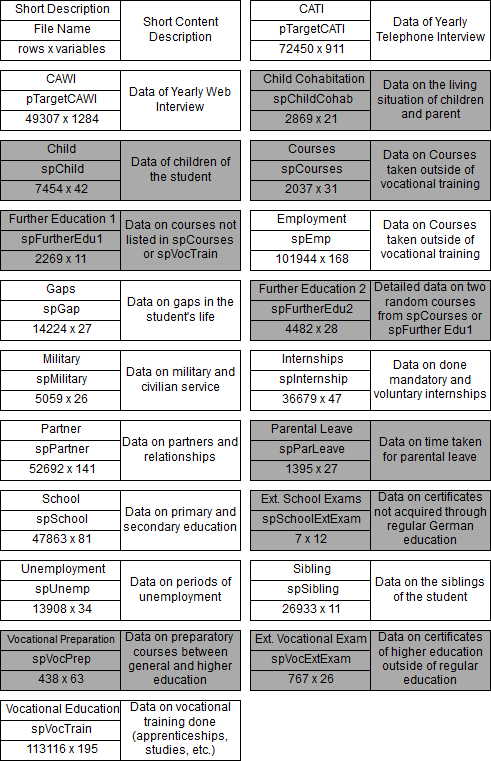
\includegraphics[width=.75\textwidth]{file_overview}
    \mycaption{Overview of used NEPS files}{An overview of all files in the NEPS dataset. Those marked in gray have not been used in the analysis.}
    \label{fig:file_overview}
\end{figure}
% \begin{description}
% 	\item [Computer Assisted Telephone Interview] CATI
% 	\item [Computer Assisted Web Interview] CAWI
% 	\item [Child] Children stuff
% 	\item [Child Cohabilitation] Living with children
% 	\item [Courses] Courses done
% 	\item [Employment] Phases of Employment
% 	\item [Further Education] Additional Education
% 	\item [Gap] Gap years done
% 	\item [Internship] Internships done
% 	\item [Military] Military and Civil Service episode
% 	\item [Parental Leave] Taken Parental Leave
% 	\item [Partner] Special Someone Information
% 	\item [School] School Education
% 	\item [School External Exams] External Examinations
% 	\item [Sibling] Siblings
% 	\item [Unemployment] Non-Employment
% 	\item [Vocational External Exam] External Exams linked to Vocational Training
% 	\item [Vocational Preperation] Ehm?
% 	\item [Vocational Training] Vocational Trainings like Higher Education and Apprenticeships
% \end{description}